%!TEX TS-program = xelatex
%!TEX encoding = UTF-8 Unicode

\chapter{ข้อมูลของสถานที่ตั้งสนามบิน \\
Aerodrome Site Details}

\section{แผนผังสนามบินที่แสดงสิ่งอำนวยความสะดวกหลัก}

ประกอบด้วย แผนผังสนามบินและสิ่งอำนวยความสะดวกหลัก และแผนผังอาคารและสิ่งอำนวยความสะดวกภายในสนามบิน ดังแสดงในรูปข้างล่าง

\subsection{แผนผังสนามบินและสิ่งอำนวยความสะดวกหลัก}

\begin{figure}[ht!]
\begin{center}
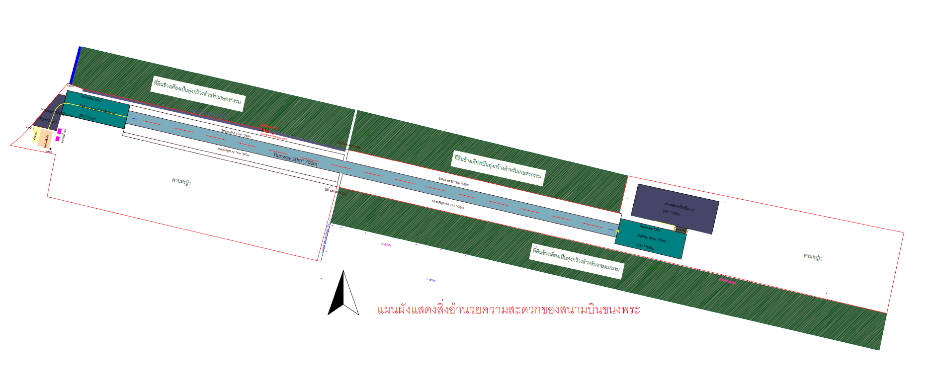
\includegraphics[scale=1.0]{Picture1.png}
\caption{แผนผังสนามบินและสิ่งอำนวยความสะดวกหลักของสนามบินขนงพระ}
\label{default}
\end{center}
\end{figure}

\newpage
\subsection{แผนผังแสดงสิ่งอำนวยความสะดวกของสนามบิน}

\begin{figure}[h!]
\begin{center}
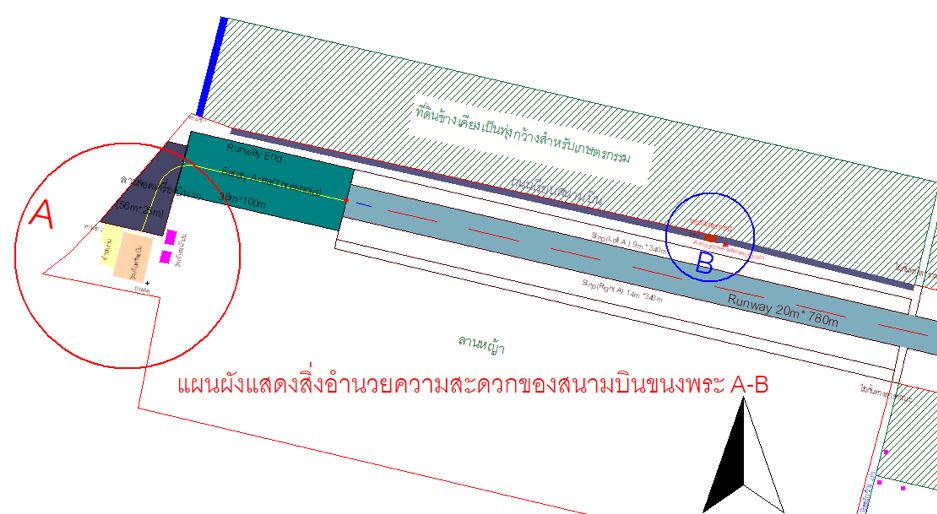
\includegraphics[scale=0.75]{Picture2.png}
\caption{แผนผังอาคารและสิ่งอำนวยความสะดวกภายในสนามบิน แสดงส่วยขยาย A และ B}
\label{default}
\end{center}
\end{figure}

\begin{figure}[h!]
\begin{center}
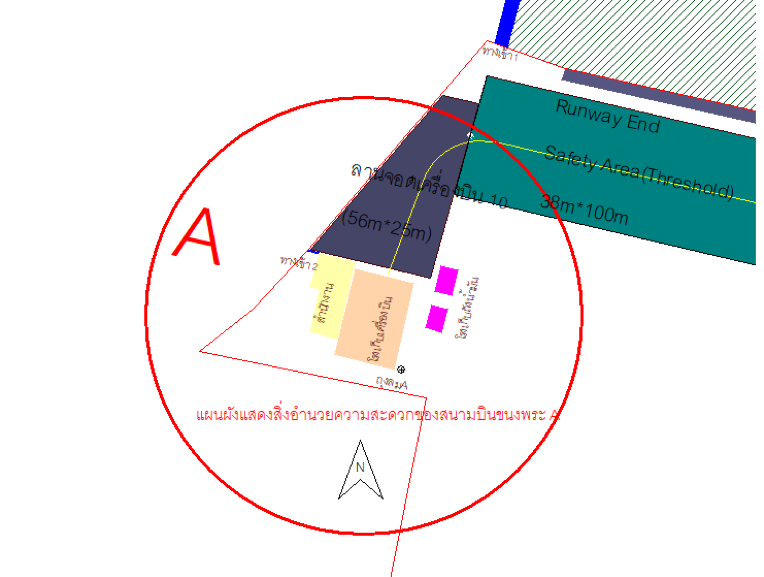
\includegraphics[scale=0.75]{Picture3.png}
\caption{แผนผังอาคารและสิ่งอำนวยความสะดวกภายในสนามบิน ขยาย A}
\label{default}
\end{center}
\end{figure}

\begin{figure}[h!]
\begin{center}
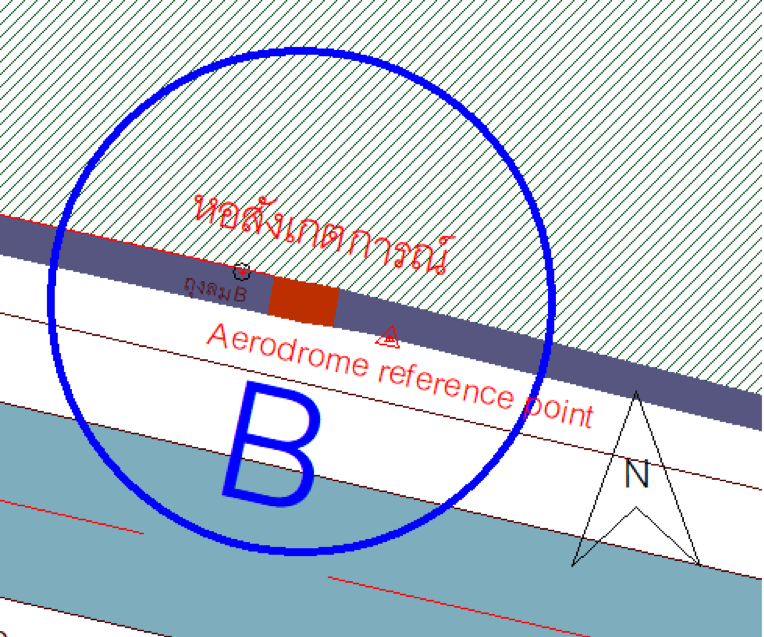
\includegraphics[scale=0.65]{Picture4.png}
\caption{แผนผังอาคารและสิ่งอำนวยความสะดวกภายในสนามบิน ขยาย B}
\label{default}
\end{center}
\end{figure}

\section{แผนผังสนามบินแสดงแนวเขตสนามบิน} \label{แผนผังสนามบินแสดงแนวเขตสนามบิน}

สนามบินขนงพระ ตั้งอยู่ในเขตอำเภอปากช่อง จังหวัดนครราชสีมา  ทิศเหนือและทิศตะวันออก เป็นไร่เกษตรกรรม ทิศใต้เป็นไร่ข้าวโพด และป่าไม้ในเขตที่ดินส่วนบุคคล  และทิศตะวันตกเป็นสนามกอล์ฟ  สนามบินมีเนื้อที่ประมาณ 160,050 ตารางเมตร หรือ 100 ไร่ (ดังรูประบายสีฟ้าข้างล่าง)                                      

\begin{figure}[h!]
\begin{center}
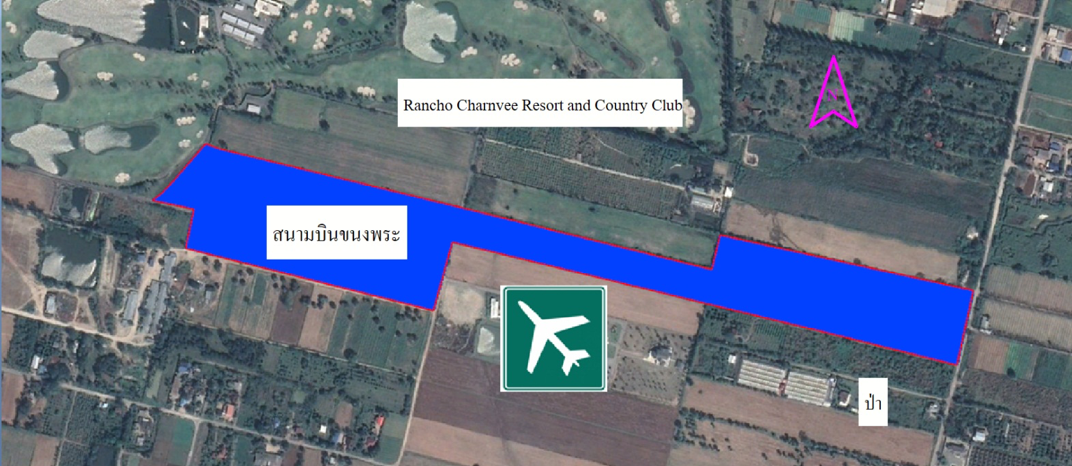
\includegraphics[width=\linewidth]{Picture5.png}
\caption{แผนผังแนวเขตสนามบินขนงพระ อำเภอปากช่อง จังหวัดนครราชสีมา}\label{แผนผังแนวเขตสนามบินขนงพระ อำเภอปากช่อง จังหวัดนครราชสีมา}
\label{default}
\end{center}
\end{figure}

\newpage
\section{แผนผังที่แสดงถึงระยะห่างของสนามบินกับเมือง}
	สนามบินขนงพระ ตั้งอยู่ ตำบลขนงพระ อำเภอปากช่อง  จังหวัดนครราชสีมา อยู่ห่างจากตัวอำเภอปากช่อง  15 กิโลเมตร 
\begin{figure}[ht!]
\begin{center}
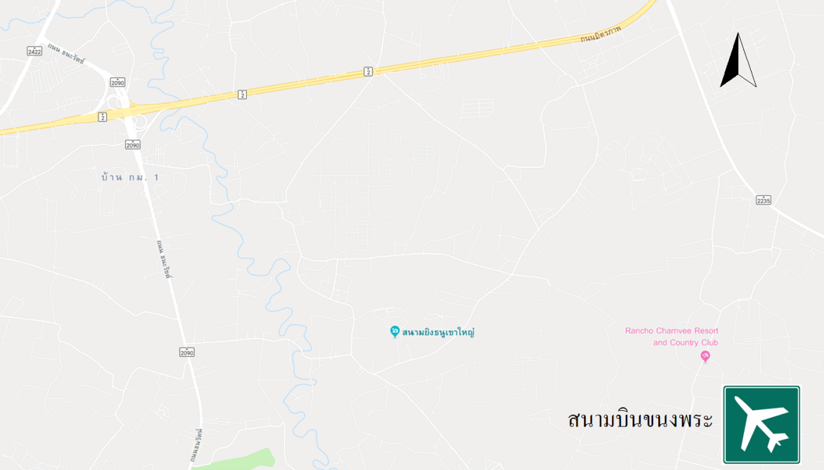
\includegraphics[width=\linewidth]{Picture6.png}
\caption{แผนผังแสดงตำแน่งที่ตั้งสนามบินขนงพระ อำเภอปากช่อง  จังหวัดนครราชสีมา}
\label{default}
\end{center}
\end{figure}

\section{หลักฐานแสดงกรรมสิทธิ์ หรือสิทธิครอบครอง หรือสิทธิใช้ประโยชน์ของที่ดิน ที่สนามบินตั้งอยู่}

สถานที่ตั้งสนามบินขนงพระประกอบไปด้วยที่ดิน 7 แปลง รายละเอียดตามภาพและตารางแสดงข้อมูลที่ดิน

\begin{figure}[htbp]
\begin{center}
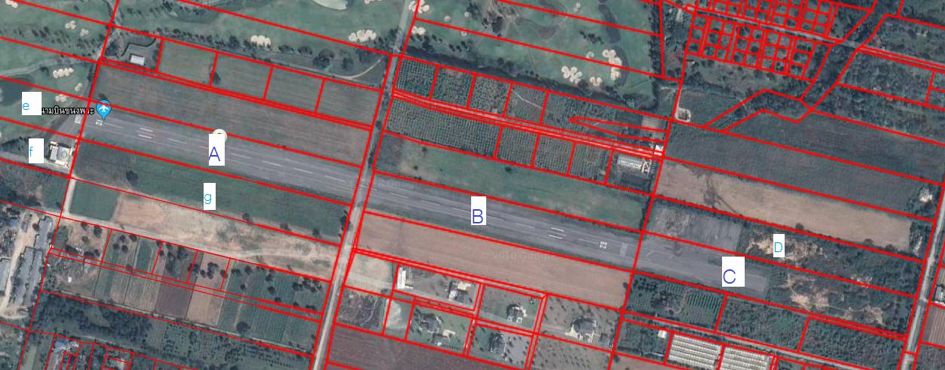
\includegraphics[width=\linewidth]{Picture7.png}
\caption{เขตแผนผังโฉนดที่ดินของสนามบินขนงพระ}
\label{default}
\end{center}
\end{figure}

โดยมีรายละเอียดโฉนดที่ดินดังนี้

\begin{enumerate}
\item กรรมสิทธิ์ที่ดินแปลงที่ A B C D และ E เป็นโฉนดที่ดิน และ นส.3 ก ของ บริษัท เจริญคีรี จำกัด โดยนางอนิลรัตน์ นิติสาโรจน์ และนางสาวปราณี พิริยะมาสกุล เป็นกรรมการผู้มีอำนาจลงนาม ได้รับทราบและยินยอมให้นายอนุทิน ชาญวีรกูล เป็นผู้มีอำนาจกระทำการใดๆ ในที่ดินจำนวน 5 แปลงของบริษัทเจริญคีรี จำกัด \footnote{รายละเอียดหนังสือยินยอมจาก บริษัท เจริญคีรี จำกัด ใน ผนวก ข. (\ref{เอกสารสิทธิ์และหนังสือยินยอมให้ใช้ประโยชน์ที่ดินจาก บริษัท เจริญคีรี จำกัด})}
\item กรรมสิทธิ์ที่ดินแปลง F และ G เป็นโฉนดที่ดินของ บริษัท กอล์ฟเขาใหญ่ จำกัด โดยนางอนิลรัตน์ นิติสาโรจน์ และนางสาวปราณี พิริยะมาสกุล เป็นกรรมการผู้มีอำนาจลงนาม ได้รับทราบและยินยอมให้นายอนุทิน ชาญวีรกูล เป็นผู้มีอำนาจกระทำการใดๆ ในที่ดินจำนวน 2 แปลงของบริษัทเจริญคีรี จำกัด \footnote{รายละเอียดหนังสือยินยอมจาก บริษัท กอล์ฟเขาใหญ่ จำกัด ใน ผนวก ข. (\ref{เอกสารสิทธิ์และหนังสือยินยอมให้ใช้ประโยชน์ที่ดินจาก บริษัท กอล์ฟเขาใหญ่ จำกัด})}
\end{enumerate}

\begin{table}[h!]
\caption{รายละเอียดกรรมสิทธิ์ที่ดิน สนามบินส่วนบุคคลขนงพระ}
\begin{center}
\begin{tabular}{|c|c|c|c|c|c|c|} %7 columns
\hline
\multirow{2}{*}{แปลงที่ดิน}  & \multicolumn{5}{c|}{เอกสารสิทธิ์ (โฉนดที่ดิน และ นส. 3ก.)} & \multirow{2}{*}{ผู้ถือกรรมสิทธิ์}  \\ \cline{2-6}
 & เลขที่ & ระวาง & เลขที่ดิน & เล่มที่ & หน้า  &   \\
 \hline
A & โฉนด 41432 & 5238 II 6418 & 166 & 415 & 32 & บริษัท เจริญคีรี จำกัด \\
B & โฉนด 35451 & 5238 II 6618, 6418 & 52 & 355 & 51 & บริษัท เจริญคีรี จำกัด \\
C & โฉนด 35572 & 5238 II 6618 & 191 & 356 & 72 & บริษัท เจริญคีรี จำกัด \\
D & นส.3ก 6322 & -- & 348 & 64ก & 22 & บริษัท เจริญคีรี จำกัด \\
E & นส.3ก 2669 & -- & 167 & 27ข & 19 & บริษัท เจริญคีรี จำกัด \\
F & โฉนด 35445 & 2538 II 6418 & 84 & 355 & 45 & บริษัท กอล์ฟเขาใหญ่ จำกัด \\
G & โฉนด 35446 & 5238 II 6418 & 85 & 355 & 51 & บริษัท กอล์ฟเขาใหญ่ จำกัด \\
\hline 
\end{tabular}
\end{center}
\label{default}
\end{table}%
